\section{Model}
We present, with theory, a comparison of two estimators for the mean of a collection of graphs.  This work considers the scenario of having M graphs represented as adjacency matrices, $A_m$, each having N vertices with known correspondence.  The graphs we consider are undirected and unweighted with no self-loops, thus each $A_m$ is a binary ($\in \{0,1\}$) symmetric matrix with zeros along the diagonal. An example scenario of this arises in the field of connectomics, where functional brain imaging data for each subject can be represented as a graph, with each vertex having a defined anatomical correspondence, and an edge between two regions is defined to exist if correlation in activity between the regions reaches a certain threshold. In this setting, we may consider each graph to be a random graph.  The general model for such graphs is the Independent Edge Model with parameter $P \in [0,1]^{N\times N}$.  Each $P_{ij}$ refers to the probability that an edge exists between vertex $i$ and vertex $j$. We aim to estimate $P$ with our finite sample of M graphs.

\subsection{Entry-Wise Least Squares Estimate}
The most intuitive approach in this scenario is the element-wise mean among the adjacency matrices:
\begin{equation}
\bar{A} = \frac{1}{M}\sum\limits_{m = 1}^M A_m
\end{equation}
In this approach each element of the adjacency matrix $A_{ij}$ is treated as an independent Bernoulli random variable with probability $P_{ij}$.  Therefore, with each element examined in isolation, to estimate the mean graph $P$ one should take the element-wise mean, $\bar{A}$.

\subsection{Model Assumption: Stochastic Block Model}
Since the number of independent edges increases on the order of $N^2$ with respect to the number of vertices, it becomes necessary to make structural assumptions on the vertices to better estimate the matrix $P$. A first structural assumption is the stochastic block model (SBM), where each vertex is assigned to a block and the probability that an edge exists between two vertices depends only on their respective block memberships.  This imposes the idea of \textit{structural equivalence}, where vertices are defined to be structurally equivalent if there connections to other nodes are similar.  In the stochastic block model, groups of vertices, or blocks, are then structurally equivalent since the vertices contained have equal likelihood in their connections among the blocks.  An example of block structure can be thought to exist in functional brain imaging, for instance the structures in the basal ganglia will likely behave similarly in their connections and may be considered a block.

The SBM is formally defined by the parameters $k$, $\rho$, and $B$. In this model each vertex is assigned to one of $k$ blocks and the fraction of vertices belonging to the $i$ th block is designated as $\rho_i$.  The connection probabilities of this block structure are stored in the symmetric $k\times k$ block matrix $B$, where $B_{ij}$ represents the probability of an edge existing between a vertex of block $i$ and one of block $j$.

\begin{figure}[!htb]
	\centering
	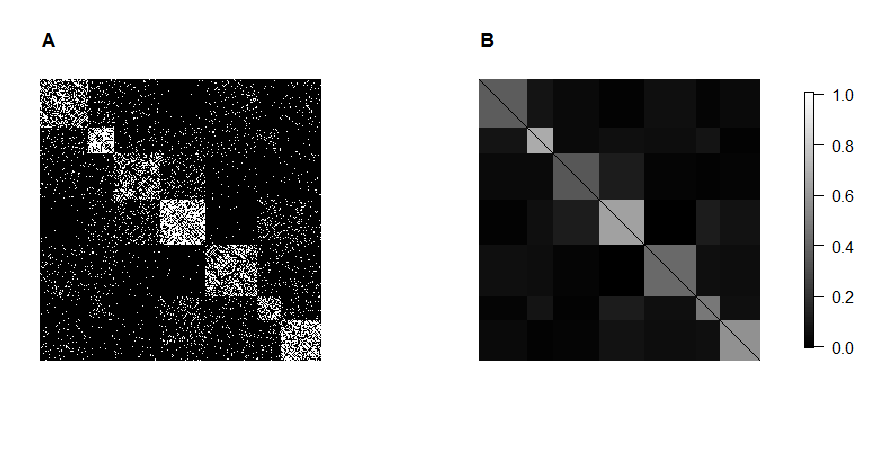
\includegraphics[width=16cm]{SBM_Example.png}
	\caption{Example illustrating the SBM. (a) Adjacency matrix generated from the (b) edge-wise probability matrix that follows a SBM with k = 7 blocks}
	\label{fig:plot1}
\end{figure}

\subsection{Latent Position Model}
In general, the SBM is too strict for applications since vertices, though they may behave similarly, often do not behave identically. A model for random graphs proposed by Hoff et. al. that can loosen this restriction is the latent position model.  In this model, each vertex has an associated latent vector, and the probability of a edge being present between two vertices is dependent only on their latent vectors. \cite{Hoff}  

A specific instance of this model that we will examine is the random dot product graph (RDPG) in which the probability of an edge being present between two nodes is the dot product of their latent vectors.\cite{Schein}.  For example in the functional connectomics, components of the latent vectors may refer the relative importance of an anatomical region among a set of tasks.  The magnitude then may refer to how active the region is generally.  Therefore, active regions vital for a similar task are more likely to be functionally connected.

In a latent position model representing a SBM, all vertices in the same block would have identical latent positions.  In the context of applications, it is unrealistic to have such a strict assumption.  However when representing the graph as an RDPG, we can relax this structure by assuming that the latent positions of vertices within a certain block are gaussian distributed around the true block latent position.  This now allows for a flexible model that can capture block-like structure in the graph while maintaining subtle distinctions among vertices within each block.

\subsection{Adjacency Spectral Embedding: $\hat{P}$}
In order to expose the underlying block structure within a graph, Sussman et. al. studied adjacency spectral embedding (ASE) to enforce a low rank$-k$ approximation on the the probability matrix P \cite{Sussman2012}.  This embedding creates a RDPG representation of the adjacency matrix from its low rank eigen decomposition.  The latent vectors are stored in the $N \times k$ matrix $X$, where the columns are comprised of the eigenvectors associated with the $k$ largest eigenvalues of the adjacency matrix.  With this embedding, $X$, each row is then a latent vector for the corresponding vertex.

In this work, we use ASE to embed the mean matrix $\bar{A}$, rather than the adjacency matrix alone.  By making the assumption that there is an underlying block-distibuted RDPG structure to graphs, enforcing this low rank approximation on $\bar{A}$ will provide a better estimate for the true mean matrix, $P$.  We will refer to this new estimate as $\hat{P}$ = $XX^T$.  Details of this algorithm are presented in section 5.

\subsection{Performance Evaluation: Relative Efficiency}
To compare the performance between $\hat{P}$ and $\bar{A}$, we examine the relative efficiency (RE), in mean squared error (MSE), among the two defined as:
\begin{equation}
RE_{ij} = \frac{MSE(\hat{P}_{ij})}{MSE(\bar{A}_{ij})}
\end{equation}
